\documentclass[a4paper]{scrartcl}
%\documentclass[a4paper]{report}

% Uncomment to optimize for double-sided printing.
% \KOMAoptions{twoside}

% Set binding correction manually, if known.
% \KOMAoptions{BCOR=2cm}

% Localization options
\usepackage[english]{babel}
\usepackage[T1]{fontenc}
\usepackage[utf8]{inputenc}

% Enhanced verbatim sections. We're mainly interested in
% \verbatiminput though.
\usepackage{verbatim}

% PDF-compatible landscape mode.
% Makes PDF viewers show the page rotated by 90°.
\usepackage{pdflscape}

% Advanced tables
\usepackage{tabu}
\usepackage{longtable}

% Fancy tablerules
\usepackage{booktabs}

% Graphics
\usepackage{graphicx}

% Current time
\usepackage[useregional=numeric]{datetime2}

% Float barriers.
% Automatically add a FloatBarrier to each \section
\usepackage[section]{placeins}

% Custom header and footer
% \usepackage{fancyhdr}
% \setlength{\headheight}{15.2pt}
% \pagestyle{fancyplain}

\usepackage{geometry}
\usepackage{layout}

\usepackage{subcaption}

% Math tools
\usepackage{mathtools}
% Math symbols
\usepackage{amsmath,amsfonts,amssymb}

% \fancyhf{}
% % Chapter header on non-plain pages only.
% \lhead{\fancyplain{} {\leftmark}}
% % Footer must contain print date. Ugly, but IPA requirement.
% \lfoot{\printdate}
% % Print date left and page count right was the thing which looked the
% % most balanced.
% \rfoot{\thepage}
% 
% Source code & highlighting
\usepackage{listings}

% Convenience commands
\newcommand{\mailsubject}{2409 - Datenstrukturen und Algorithmen - Serie 1}
\newcommand{\maillink}[1]{\href{mailto:#1?subject=\mailsubject}
                               {#1}}

% Should use this command wherever the print date is mentioned.
\newcommand{\printdate}{\today}

\subject{2409 - Datenstrukturen und Algorithmen}
\title{Series 1, Practical Exercises}

\author{Michael Senn}

\date{}

% Needs to be the last command in the preamble, for one reason or
% another. 
\usepackage{hyperref}


\begin{document}
\maketitle

% \tableofcontents

\section*{Exercise 1}

All measurements were performed on a notebook with an Intel i7-7500U CPU @ 2.7 GHz.

\subsection*{Runtime of insert-sort}

As seen in the graph below, runtime of insert sort has grown rougly
exponentially with rising number of samples to sort. This matches well with the
theory, namely its worst- and average-case complexity of O($n^2$).

\subsubsection*{Estimate of runtime for bigger sample sizes}

With its runtime complexity of O($n^2$), the runtime of this algorithm can be
expressed as $t = c * n^2$ for a given constant $c$. This allows us to estimate
this constant based on measurements taken.
\\

\begin{tabular}{|l|c|c|c|c|c|c|}
	\hline
	Sample count & 10000 & 30000 & 50000 & 1000000 & 300000 & 500000 \\
	Runtime [s] & 0.026 & 0.145 & 0.372 & 1.511 & 14.379 & 44.486 \\
	c ($ * 10^{-10}$)& 2.6 & 1.61 & 1.49 & 1.51 & 1.60 & 1.78 \\
	\hline
\end{tabular}
\\

In order to minimize the impact of timing inaccuracies - as well as other
sources of variance - influencing the measurements with fewer samples, we used
a weighted average to calculate the constant, using the number of samples as a
weight. This leads to a weighted average of $1.69 * 10^{-10}$.

Using this constant, the runtime to sort 10 million samples can be estimated to
be in the range of 16900 seconds - roughly 4h 42min.

\subsection*{Runtime of merge-sort}

As seen in the graph below, runtime of merge sort has grown rougly linearly
with rising number of samples to sort. While we would expect slightly
faster-than-linear growth due to its worst- and average-case complexity of O($n
* log(n)$), that difference is hard to observe for relatively small sample
sizes - made worse by the inaccuracies introduced due to the way execution time
was measured.

\begin{figure}
    \centering
    \begin{subfigure}{.5\textwidth}
      \centering
      \caption{Runtime of insert-sort}
      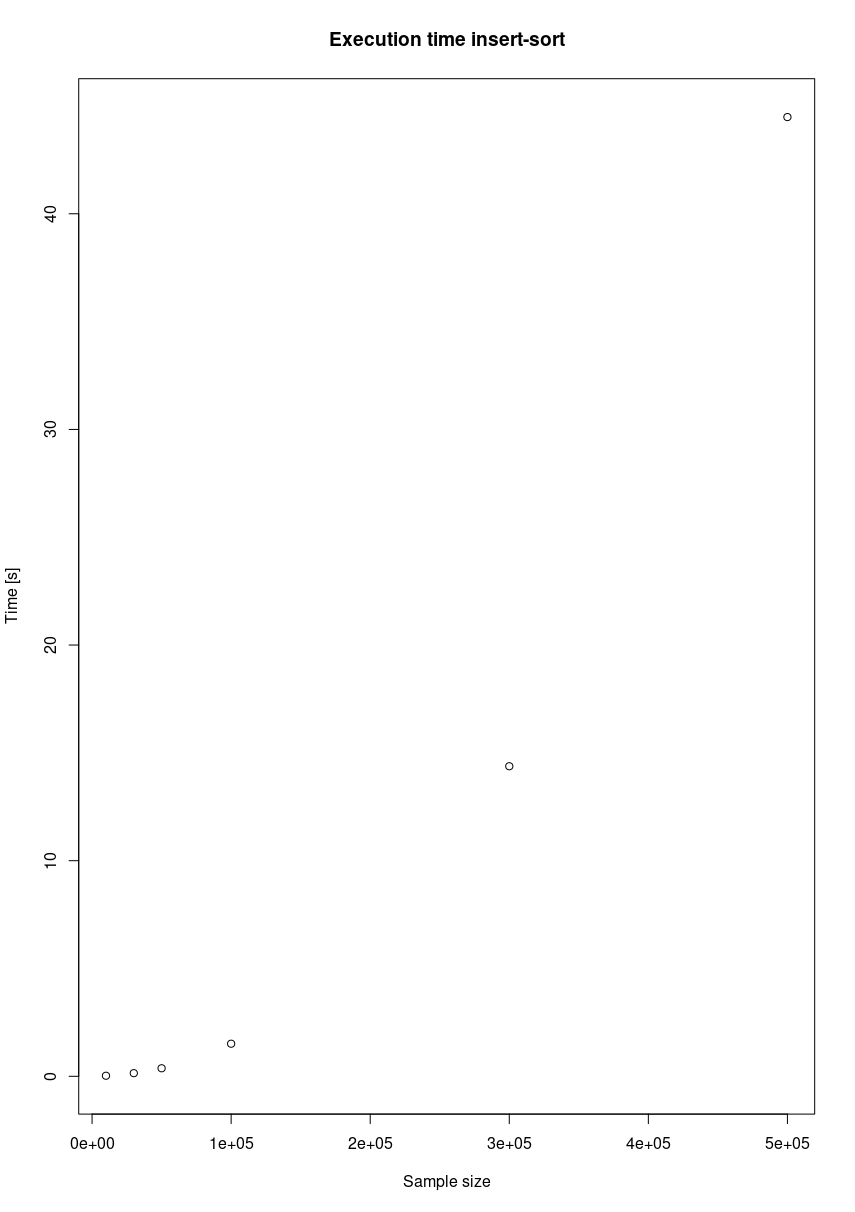
\includegraphics[width=\linewidth]{resources/insert_sort.png}
    \end{subfigure}%
    \begin{subfigure}{.5\textwidth}
      \centering
      \caption{Runtime of merge-sort}
      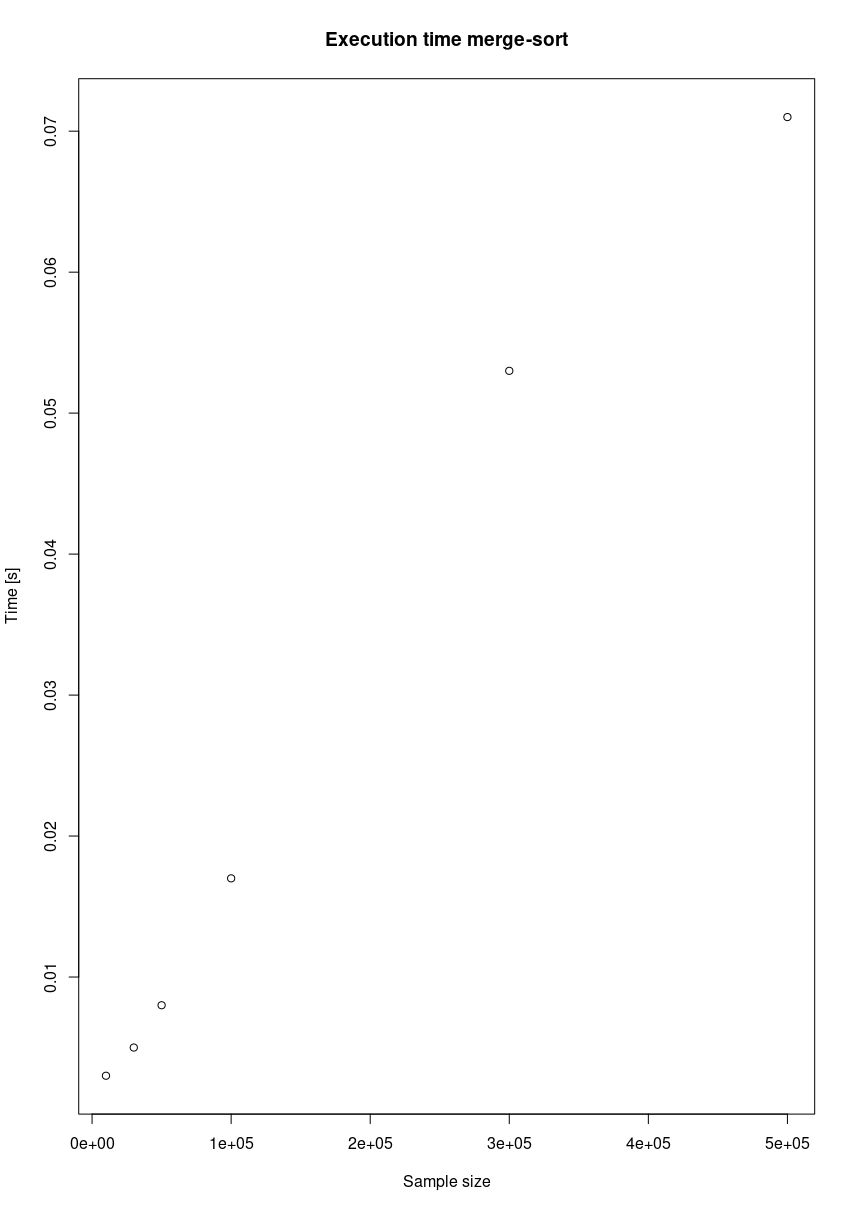
\includegraphics[width=\linewidth]{resources/merge_sort.png}
    \end{subfigure}
\end{figure}

\end{document}
